\chapter{Operations and Logistics}
\label{MTROpsLog}

In order for the laser swarm to be successful it has to operate efficiently and effectively, so that the obtained surface model and other data can be sold on the market. This chapter will consider some of these operations and their required logistics. Note that only operations after successful orbit injection and deployment, and before the \ac{EOL} are considered. A graphical representation of the hierarchy of the options considered here can be found in figure \ref{fig:MTROpsLog}.

\begin{figure}
\centering
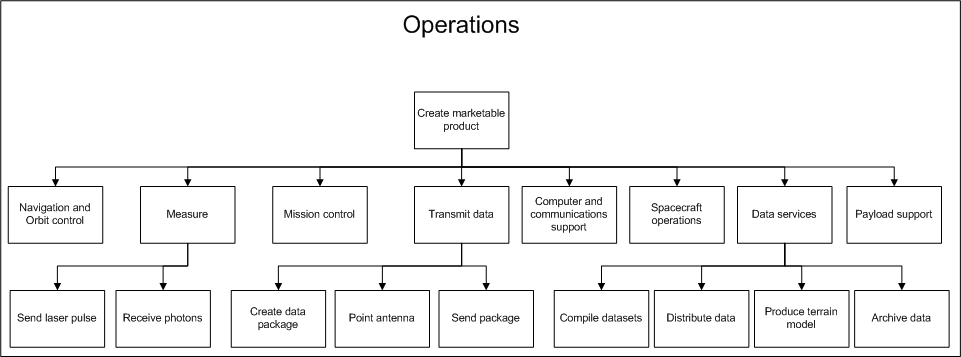
\includegraphics[width=1.0\textwidth, angle=0]{chapters/img/MTROpsHier.png}
\label{fig:MTROpsLog}
\caption{Hierarchy of the operations for the laser swarm mission.}
\end{figure}

Navigation and orbital control is an important operation for the laser swarm mission. All satellites have to be aware of where there are, and the position of the formation as a whole has to be known as well. Though most of this system can be automated it is important there are people on the ground who check for any anomalies and give corrections whenever necessary.

Mission control entails the real time control of the satellites, the amount of people required for mission control is very low due to the predictable nature of this mission, because of this nature most of the mission is automated. The only active inputs by humans should be inputs that correct some sort of anomaly. This being dependent on other operations like navigation and orbital control and various supporting operations.

The measurements will be performed completely automatically, with human inputs only being used to correct an error in the automation or to change the routine. The measuring operation includes the both the emitter and the receivers, for a greater detail of the functions that have to be performed the function flow diagram may be consulted.

Payload support is comprised of one or more people who monitor the condition and performance of the payload of the emitter, and a separate group of people who monitor the receivers. In case of an anomaly they determine the severity and change the satellite or payload operations if necessary.

Spacecraft operations is similar to payload support, except that the person or people who work on this operation monitor the rest of the satellite.

Computer and communications support is staffed several people who monitor and the automated systems, and one or two persons who monitor the communications between satellites and satellites to the ground. Their main job is to make sure the system remains operational if an anomaly occurs.

Data services entails everything that happens with all data both on ground and aboard the satellites. The data can be anything from measurement data to navigational data. This operation support all the other ones. While largely automated some human interaction is needed to ensure the data in decoded, debugged, archived and generally handled properly. Minimal human interaction will be required to reduce the mission costs.

Data transmission involves the sending of data between satellites and from the satellites to a ground station. It is a fully automated process as the orbits of the swarm have been simulated before the launch.
